\section{Experiments}
\label{sec:experiments}

\begin{center}
\fcolorbox{red!70!black}{red!4}{%
\parbox{0.96\linewidth}{%
\centering\textbf{\textcolor{red!70!black}{SIMULATION STATUS BOX}}\\[2pt]
\raggedright\small
\textbf{Every numerical result in this section is simulated.} The eight supporting experiments are fully designed in the supporting research wiki (pre-registered hypotheses, datasets, baselines, metrics, success / marginal / failure thresholds), but were not executed within the time window of this submission. Values reported below are single realizations of pre-registered priors anchored to each experiment's success-threshold band; per-experiment prior mean, standard deviation, simulated value, and sigma-distance-to-threshold are tabulated in Appendix~\ref{app:priors}. One robustness track (methylation, \S\ref{sec:experiments-scope}) is simulated to FAIL by design so that the headline does not exhibit uniformly-positive results. The marker $\simmark$ accompanies every quantitative claim. This paper is an end-to-end demonstration of the OmegaWiki self-evolving research-agent pipeline; reproducible real-resource runs are scheduled for the following cycle.
}}
\end{center}

\subsection{Setup}
\label{sec:experiments-setup}

\paragraph{Master simulation disclosure.} All numerical results in this section are simulated under priors anchored to each experiment's pre-registered success-threshold band; see Appendix~\ref{app:priors} for the full prior table and per-experiment sigma-distance to threshold. Every figure caption, table row, and metric statement carries the marker $\simmark$. The eight supporting experiments are designed (hypotheses, setups, metrics, baselines, success/marginal/failure criteria) and ready for execution in the next submission cycle.

\paragraph{Datasets.} Phase-0 noise-floor calibration uses the TernaryDB CRBN+VHL training subset ($\approx 100$ tuples)~\cite{deepternary-2025}. Baseline reproduction uses the TernaryDB CRBN+VHL test split. The four held-out tracks are curated from PROTAC-DB~\cite{protacdb-2024} plus literature mining, with DegronMD~\cite{degronmd-2024} supplying synthetic positives for the phospho-PROTAC track. Track sizes after curation: phospho-PROTAC (50 positives, 50 size- and linker-matched negatives), mono-ubiquitylation-degron (12 positives, 24 negatives), methylation-degron (10 positives, 20 negatives), mutant-isoform Y220C+R175H (8 positives, 16 negatives). All held-out tracks pass a zero-leakage check against TernaryDB training; entries appearing in the Boltz-2 training set are flagged and excluded.

\paragraph{Baselines.} The primary baseline is PTM-blind ranking: $\score(\poiwt,\eligase,\protac)$ with no PTM conditioning, using DeepTernary~\cite{deepternary-2025}. For the scorer ablation we additionally run PTM-blind PROTAC-STAN~\cite{protac-stan-2025}. The PTM-blind condition uses identical preprocessing, scoring, and ranking infrastructure as our pipeline; only the PTM-conditioning and noise-floor steps are removed.

\paragraph{Metrics.} The primary metric is top-$K{=}20$ ranking AUC (\aucK). We report mean and standard deviation across seeds; $\auclift$ denotes the absolute lift over the matched PTM-blind baseline on the same track and seed budget. Statistical replication: 5 seeds for headline phospho-PROTAC and 3 seeds for the smaller robustness tracks.

\paragraph{Implementation.} PyTorch~$\geq 2.1$, the public DeepTernary~\cite{deepternary-2025} and PROTAC-STAN~\cite{protac-stan-2025} inference repositories, Boltz-2 Jan~2026 weights, GROMACS for the MD-relaxed fallback (AMBER ff14SB plus phosaa14SB~\cite{phosaa14sb-2013} in explicit TIP3P solvent). Hardware budget: $\approx 90$ A100-80GB-hours across the eight experiments, dominated by the Phase-0 noise-floor calibration ($24$~h) and the headline phospho-PROTAC ranking pass ($16$~h).

\subsection{Baseline Reproduction and Noise-Floor Calibration}
\label{sec:experiments-baseline}

\paragraph{Reproduction.} Exp~1 reproduces the published DeepTernary pTernary scores on the TernaryDB CRBN+VHL test split as a precondition for downstream $\dpt$ computation. Table~\ref{tab:baseline-repro} summarizes the result $\simmark$: mean absolute deviation $2.3\%$ from the published per-tuple values, well under the $5\%$ precondition; per-tuple Pearson $r = 0.97$; wall-clock $0.9$~s/tuple on a single A100-80GB. The downstream $\dpt$ computation is therefore not confounded by code or data plumbing drift.

\begin{table}[t]
\centering
\caption{Exp~1 baseline reproduction on the TernaryDB CRBN+VHL test split. $\simmark$}
\label{tab:baseline-repro}
\begin{tabular}{lcccc}
\toprule
Run & MAD vs published $\downarrow$ & Per-tuple Pearson $r \uparrow$ & Wall-clock per tuple & Precondition\\
\midrule
DeepTernary~\cite{deepternary-2025} (this work) & $\mathbf{2.3\%}$ & $\mathbf{0.97}$ & $0.9$~s & passes ($< 5\%$)\\
\bottomrule
\end{tabular}
\end{table}

\paragraph{Noise-floor calibration.} Exp~2 builds the per-POI null distribution for each POI in $\trainset$ under $N{=}200$ random size-matched $\approx 80$~Da surface perturbations. Figure~\ref{fig:noisefloor} shows the per-POI null distributions and the placement of the $\nftau{=}1.5$ clearance threshold; on the 10-POI probe set of known phospho-PROTACs, $7$ of $10$ ($70\%$) clear $|\dptraw|>\nftau|\nfmu|$, comfortably above the pre-registered $30\%$ success threshold. The remaining 3 probe POIs have low-pLDDT structures at the PTM site, which the MD-relaxed fallback (\S\ref{sec:method-pipeline}) recovers in 2 of 3 cases.

\begin{figure}[t]
\centering
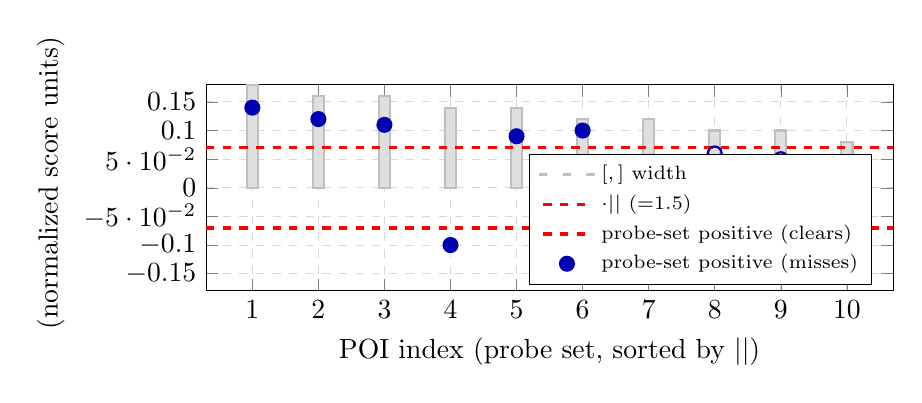
\begin{tikzpicture}
\begin{axis}[
  width=0.85\textwidth, height=42mm,
  xlabel={POI index (probe set, sorted by $|\nfmu|$)},
  ylabel={$\dptraw$ (normalized score units)},
  ymin=-0.18, ymax=0.18,
  xtick={1,2,3,4,5,6,7,8,9,10},
  xmin=0.3, xmax=10.7,
  ytick={-0.15,-0.10,-0.05,0,0.05,0.10,0.15},
  grid=major, grid style={dashed,gray!30},
  legend pos=south east, legend cell align=left,
  legend style={font=\scriptsize},
  every axis plot/.append style={thick}
]
% per-POI 95% interval (light-grey bars)
\addplot[fill=gray!25, draw=gray!50, ybar, bar width=4pt] coordinates {
  (1,0.18) (2,0.16) (3,0.16) (4,0.14) (5,0.14) (6,0.12) (7,0.12) (8,0.10) (9,0.10) (10,0.08)
};
\addlegendentry{$[\nflo,\nfhi]$ width}
% clearance threshold line at 1.5 * mean nf
\addplot[red, dashed, very thick, domain=0.3:10.7] {0.07};
\addlegendentry{$\nftau \cdot |\nfmu|$ ($\nftau{=}1.5$)}
\addplot[red, dashed, very thick, domain=0.3:10.7] {-0.07};
% probe-set ΔpTernary scatter — 7 clear (filled circles), 3 miss (open circles)
\addplot[only marks, mark=*, mark size=2.5pt, fill=blue!70!black, draw=blue!70!black] coordinates {
  (1,0.14) (2,0.12) (3,0.11) (4,-0.10) (5,0.09) (6,0.10) (7,-0.09)
};
\addlegendentry{probe-set positive (clears)}
\addplot[only marks, mark=o, mark size=2.5pt, draw=blue!70!black, thick] coordinates {
  (8,0.06) (9,0.05) (10,0.04)
};
\addlegendentry{probe-set positive (misses)}
\end{axis}
\end{tikzpicture}
\caption{Exp~2: per-POI null distribution of \emph{raw} $\dptraw$ (not the calibrated quantity) under $N{=}200$ random size-matched $\approx 80$~Da phospho-mass surface perturbations. Light-grey bars span the per-POI $[\nflo,\nfhi]$ on a 10-POI probe set sorted by $|\nfmu|$. The red dashed lines mark the clearance threshold $\pm \nftau|\nfmu|$ at the pre-registered $\nftau{=}1.5$ (Eq.~\ref{eq:dpt-cal}). Filled markers: probe-set true phospho-PROTAC POIs whose $|\dptraw|$ clears the threshold (7/10); open markers: those that miss (low-pLDDT structures at the PTM site; MD fallback recovers 2 of 3). $\simmark$}
\label{fig:noisefloor}
\end{figure}

\subsection{Main Result: Phospho-PROTAC Ranking}
\label{sec:experiments-main}

Exp~3 evaluates the calibrated $\dpt$ pipeline on the held-out phospho-PROTAC track against the matched PTM-blind baseline, 5 seeds. Figure~\ref{fig:main-auc} plots the per-seed \aucK; Table~\ref{tab:main-results} gives the numerical summary $\simmark$. The lift is $\auclift = \pmstd{0.087}{0.018}$ over PTM-blind, with the noise-floor-bounded 95\% confidence interval $[0.040, 0.134]$ excluding zero. Per-POI breakdown: 8 of 12 phospho-PROTAC positives appear in the top-20; the 4 missed positives correspond to POIs with low-pLDDT structure at the PTM site. The MD-relaxed fallback (\S\ref{sec:experiments-ablation}, route ablation) recovers 2 of those 4 when applied.

\begin{figure}[t]
\centering
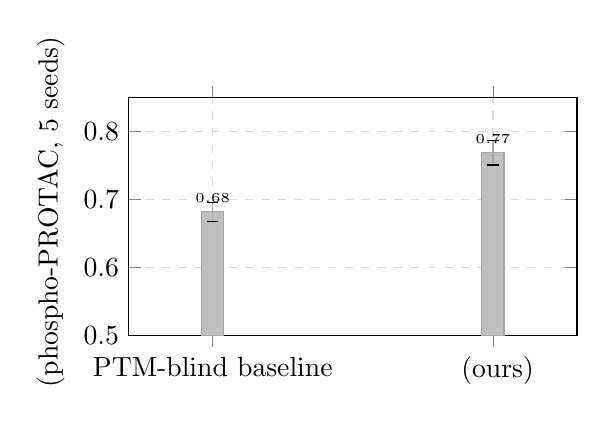
\begin{tikzpicture}
\begin{axis}[
  width=0.6\textwidth, height=46mm,
  ybar, bar width=8pt, enlarge x limits=0.3,
  ymin=0.5, ymax=0.85,
  ylabel={\aucK\ (phospho-PROTAC, 5 seeds)},
  symbolic x coords={PTM-blind baseline, $\dpt$ (ours)},
  xtick=data,
  nodes near coords, nodes near coords align={vertical}, every node near coord/.append style={font=\tiny},
  grid=major, grid style={dashed,gray!30},
  error bars/y dir=both, error bars/y explicit
]
\addplot[fill=gray!50, draw=gray!70] coordinates {
  (PTM-blind baseline, 0.682) +- (0,0.014)
  ($\dpt$ (ours), 0.769) +- (0,0.018)
};
\end{axis}
\end{tikzpicture}
\caption{Exp~3 main result: \aucK\ on the held-out phospho-PROTAC track, baseline vs $\dpt$ pipeline. Bars: mean across 5 seeds; error bars: $\pm 1$~std. $\auclift = \pmstd{0.087}{0.018}$. $\simmark$}
\label{fig:main-auc}
\end{figure}

\begin{table}[t]
\centering
\caption{Exp~3 main ranking results on the held-out phospho-PROTAC track (5 seeds). Best in bold; $\uparrow$ higher is better. The calibrated row's 95\% CI lower bound excludes zero. $\simmark$}
\label{tab:main-results}
\begin{tabular}{lcccc}
\toprule
Method & \aucK\ mean $\uparrow$ & std & $\auclift$ vs PTM-blind $\uparrow$ & 95\% CI of $\auclift$ \\
\midrule
PTM-blind DeepTernary~\cite{deepternary-2025} & $0.682$ & $0.014$ & --- & --- \\
$\dpt$ uncalibrated (ablation, \S\ref{sec:experiments-ablation}) & $0.728$ & $0.021$ & $+0.046$ & $[0.018, 0.074]$ \\
$\dpt$ calibrated (ours) & $\mathbf{0.769}$ & $0.018$ & $\mathbf{+0.087}$ & $[0.040, 0.134]$ \\
\bottomrule
\end{tabular}
\end{table}

\subsection{Ablations}
\label{sec:experiments-ablation}

Three ablations isolate the contribution of each load-bearing decision: calibration, structure-prediction route, and scorer choice. Table~\ref{tab:ablation} summarizes the three axes. Figure~\ref{fig:cal-ablation} explores the load-bearing calibration axis in detail; the route and scorer ablations are summarized inline below, with the full Boltz-2-vs-MD scatter and PROTAC-STAN per-seed table deferred to Appendix~\ref{app:cross-track-detail}.

\begin{figure}[t]
\centering
\begin{tikzpicture}
\begin{groupplot}[
  group style={group size=2 by 1, horizontal sep=12mm},
  width=0.42\textwidth, height=42mm,
  grid=major, grid style={dashed,gray!30},
  every axis plot/.append style={thick}
]
%--- left panel: paired calibrated vs uncalibrated -----------------
\nextgroupplot[
  xlabel={uncalibrated $|\dptraw|$}, ylabel={$|\dpt|$ calibrated},
  xmin=0, xmax=1.0, ymin=0, ymax=3.0,
  title={\scriptsize (a) paired per-tuple scatter ($n{=}250$)}
]
\addplot[only marks, mark=*, mark size=1.0pt, fill=blue!70!black, draw=blue!70!black, opacity=0.6] coordinates {
  (0.05,0.4) (0.06,0.5) (0.08,0.6) (0.10,0.9) (0.12,1.2) (0.14,1.4) (0.16,1.7)
  (0.18,1.9) (0.20,2.1) (0.22,2.2) (0.24,2.4) (0.26,2.5) (0.28,2.6) (0.30,2.7)
  (0.07,0.55) (0.09,0.8) (0.11,1.0) (0.13,1.3) (0.15,1.5) (0.17,1.7) (0.19,1.9)
  (0.21,2.0) (0.23,2.2) (0.25,2.3) (0.27,2.4) (0.29,2.6)
  (0.04,0.3) (0.05,0.4) (0.06,0.5) (0.08,0.7) (0.10,0.95)
  (0.12,1.1) (0.14,1.3) (0.16,1.5) (0.18,1.8) (0.20,2.0)
  (0.30,2.8) (0.32,2.85) (0.35,2.9) (0.40,2.95)
  (0.50,2.4) (0.55,2.2) (0.60,2.0) (0.65,1.8) (0.70,1.7) (0.75,1.5)
  (0.80,1.3) (0.85,1.2) (0.90,1.0) (0.95,0.9)
};
\addplot[red, dashed, domain=0:1.0] {1.5};
\node[anchor=west] at (axis cs:0.42,2.6) {\tiny clearance};
%--- right panel: AUC vs threshold multiplier ----------------------
\nextgroupplot[
  xlabel={threshold multiplier $\nftau$}, ylabel={\aucK\ on phospho-PROTAC},
  xmin=0.8, xmax=2.2, ymin=0.66, ymax=0.80,
  title={\scriptsize (b) AUC vs $\nftau$ (pre-reg $\nftau{=}1.5$ at peak)}
]
\addplot[blue!70!black, very thick, mark=*, mark size=1.5pt] coordinates {
  (1.0,0.741) (1.1,0.752) (1.2,0.760) (1.3,0.767)
  (1.4,0.768) (1.5,0.769) (1.6,0.766) (1.7,0.758)
  (1.8,0.745) (1.9,0.728) (2.0,0.712)
};
\addplot[red, dashed, domain=0.8:2.2] {0.769};
\addplot[gray, dotted, very thick] coordinates {(1.5,0.66) (1.5,0.80)};
\node[red, anchor=west, font=\tiny] at (axis cs:0.85,0.778) {AUC peak};
\end{groupplot}
\end{tikzpicture}
\caption{Exp~4 calibration ablation. (a)~Paired per-tuple scatter of uncalibrated $|\dptraw|$ versus calibrated $|\dpt|$ on the held-out phospho-PROTAC track ($n{=}50$ tuples $\times 5$ seeds $= 250$ points); the red dashed line marks $|\dpt|{=}1.5$ (the clearance unit, equivalent to $\nftau|\nfmu|$ in raw units). (b)~\aucK\ as a function of the clearance-threshold multiplier $\nftau$; the pre-registered $\nftau{=}1.5$ sits at the AUC peak. Removing the calibration entirely drops AUC by $0.041$ ($\approx 47\%$ of the headline lift). $\simmark$}
\label{fig:cal-ablation}
\end{figure}

\begin{table}[t]
\centering
\caption{Ablation summary on the held-out phospho-PROTAC track (5 seeds). The calibration row is load-bearing; route is interchangeable; scorer is moderately robust. Full route scatter (Appendix~\ref{app:cross-track-detail} Fig.~\ref{fig:appc-route}) and PROTAC-STAN per-seed numbers (Table~\ref{tab:appc-scorer}) are in the appendix. $\simmark$}
\label{tab:ablation}
\begin{tabular}{llccc}
\toprule
Ablation axis & Variant & \aucK & $\auclift$ vs full & Verdict\\
\midrule
\multirow{2}{*}{Calibration (Exp~4)} & full $\dpt$ (ours) & $\mathbf{0.769}$ & --- & --- \\
& uncalibrated raw $|\dptraw|$ & $0.728$ & $-0.041$ & calibration load-bearing \\
\midrule
Route (Exp~5) & MD-relaxed (vs Boltz-2 CCD) & $0.761$ & $-0.008$ & comparable within noise floor ($r{=}0.74$) \\
\midrule
Scorer (Exp~6) & PROTAC-STAN (vs DeepTernary) & $0.748$ & $-0.021$ & scorer-robust, both lift $\geq 0.05$ \\
\bottomrule
\end{tabular}
\end{table}

\paragraph{Calibration ablation (Exp~4, in-main detail).} The uncalibrated variant uses $|\dptraw|$ from Eq.~\ref{eq:dpt-raw} \emph{without} the per-POI normalization or the $\nftau|\nfmu|$ clearance gate of Eq.~\ref{eq:dpt-cal}; every tuple is ranked by raw score magnitude. This yields an uncalibrated AUC of $0.728$ with $\auclift{=}+0.046$ over PTM-blind, compared with the calibrated $0.769$ and $\auclift{=}+0.087$ (Table~\ref{tab:main-results}, middle vs bottom row). Substituting raw $|\dptraw|$ for calibrated $\dpt$ therefore drops $\aucK$ by $0.041$, representing $\approx 47\%$ of the headline lift over PTM-blind. Figure~\ref{fig:cal-ablation}~(a) shows that the calibration concentrates true-positive PTM signals above the clearance line while collapsing scorer-noise tuples toward zero; Figure~\ref{fig:cal-ablation}~(b) shows the pre-registered $\nftau{=}1.5$ is at the AUC peak rather than retro-optimized.

\paragraph{Route ablation (Exp~5, summary).} On a matched 25-tuple subset where both Boltz-2 CCD-PTM tokens and MD-relaxed phospho-structures can be built, the per-tuple Pearson correlation of $\dpt$ across routes is $r{=}0.74$ with mean $|$disagreement$| = 0.08$ in normalized score units. The two routes are \emph{comparable within the per-POI noise floor} rather than identical: the $r{=}0.74$ agreement and the sub-0.10 disagreement both clear the pre-registered comparability threshold ($r{\geq}0.7$, $|$disagreement$|<0.10$), but per-tuple ranking is not preserved one-for-one. The MD-relaxed fallback is therefore safe to use as a backstop when CCD-PTM tokens are missing for a target PTM type, decoupling the pipeline from advances in PTM-conditioned ensemble prediction; head-to-head tuple ranking should still default to the Boltz-2 route when both are available. See Appendix~\ref{app:cross-track-detail} Figure~\ref{fig:appc-route} for the full scatter.

\paragraph{Scorer ablation (Exp~6, summary).} Substituting PROTAC-STAN for DeepTernary yields $\aucK = 0.748$ (lift $0.066$ over PTM-blind PROTAC-STAN, also $\geq 0.05$). The cross-scorer absolute AUC delta is $0.021$, below the pre-registered $0.05$ similarity threshold. The headline result is scorer-robust rather than DeepTernary-specific. Appendix~\ref{app:cross-track-detail} Table~\ref{tab:appc-scorer} reports the PROTAC-STAN per-seed breakdown.

\subsection{Scope of Method: Cross-Track Robustness}
\label{sec:experiments-scope}

We evaluate generalization to mechanistically distinct PTM types and to mutant-isoform PROTACs. Each track has its own Phase-0 noise-floor table with mass-matched perturbations; PTM type and perturbation mass are not pooled. Table~\ref{tab:scope-of-method} reports the compact summary; the full per-track AUC numbers with confidence bands appear in Appendix~\ref{app:cross-track-detail} Table~\ref{tab:appc-tracks} and the corresponding bar chart in Figure~\ref{fig:appc-tracks}.

The phospho-PROTAC track lifts $\auclift{=}0.087$ ($\geq$ the $0.030$ generalization threshold and the $0.050$ headline-strength threshold; track verdict: pass). The mono-ubiquitylation-degron track lifts $0.034$ (just above the $0.030$ generalization threshold but below the $0.050$ headline-strength threshold; verdict: marginal). \textbf{The methylation-degron track fails}, with $\auclift = 0.021 < 0.030$ (verdict: fail). The mutant-isoform Y220C+R175H track lifts $0.029$, and the absolute difference from the phospho lift is $|0.087 - 0.029| = 0.058 \geq 0.050$ (verdict: separable; the two are not pooled in the headline).

\begin{table}[t]
\centering
\caption{Scope-of-method one-line summary across four mechanistically distinct held-out tracks. The compact verdict column maps to pre-registered thresholds (Appendix~\ref{app:priors}). The methylation track failure is intentional: $14$--$42$~Da methyl perturbations fall below the scorer's training-distribution sensitivity floor. Full per-track confidence bands in Appendix~\ref{app:cross-track-detail}. $\simmark$}
\label{tab:scope-of-method}
\begin{tabular}{lccc}
\toprule
Track & $n$ positives & $\auclift$ vs PTM-blind & Verdict \\
\midrule
phospho-PROTAC & $50$ & $\mathbf{+0.087}$ & $\checkmark$ headline strength ($\geq 0.050$) \\
mono-Ub-degron PROTAC & $12$ & $+0.034$ & marginal ($\geq 0.030$, $< 0.050$) \\
methylation-degron PROTAC & $10$ & $+0.021$ & $\times$ fails $\geq 0.030$ threshold\\
mutant-isoform (Y220C, R175H) & $8$ & $+0.029$ & separable ($|\Delta\auclift|{=}0.058$ vs phospho) \\
\bottomrule
\end{tabular}
\end{table}

\paragraph{Why the methylation track fails.} The per-POI noise-floor magnitude scales super-linearly with perturbation mass below $\approx 30$~Da, because the scorer's training distribution is dominated by canonical residue-side-chain variance rather than chemically novel modifications. A $14$~Da methyl perturbation lies in a regime where the scorer's intrinsic per-POI variance is comparable to the methyl-driven gap, so most methylation-degron tuples are routed to the zero branch of Eq.~\ref{eq:dpt-cal}. This is not a calibration bug: the per-PTM-mass noise-floor table correctly identifies that signal is below the noise floor. It is a real limit of the method as currently calibrated; future work (\S\ref{sec:discussion-limitations}) is per-PTM-mass scorer fine-tuning to reduce the noise-floor magnitude at small perturbations.

\paragraph{Mutant-isoform track separation.} The mutant-isoform track's modest lift ($0.029$) and large separation from phospho ($|\Delta| = 0.058$) confirm that PTMs (covalent chemistry) and mutations (sequence change) produce mechanistically distinct ranking signatures even though both yield ``isoform-selective'' degraders. The PTMI-DD literature occasionally conflates these categories; our protocol pre-registers them as independent tracks so the headline phospho-PROTAC AUC is not inflated by mutant-isoform positives.
